
%% Creator David Li
% Modified matlab xsl latex template file to suit needs
% Use find and replace 
%		\ensuremath with ''
%		
%	    \{ with { and \} with }
% This LaTeX was auto-generated from an M-file by MATLAB.
% To make changes, update the M-file and republish this document.

\documentclass[12pt]{article}
\usepackage[utf8]{inputenc}
\usepackage{graphicx}
\usepackage{epstopdf}
\usepackage{color}
\usepackage{xcolor}
\usepackage{amsmath}
\usepackage[ocgcolorlinks]{hyperref}
\usepackage{bookmark}
\usepackage[hmargin=0.25cm,vmargin=0.25cm]{geometry}
\usepackage{fancyhdr}
\usepackage{booktabs}
\sloppy
\definecolor{lightgray}{gray}{0.5}
% \definecolor{myText}{HTML}{2B2B2B}
\definecolor{fontColor}{HTML}{171717}
\setlength{\parindent}{0pt}

\makeindex

\usepackage{listings}
\definecolor{mygreen}{RGB}{28,172,0} % color values Red, Green, Blue
\definecolor{mylilas}{RGB}{170,55,241}
\lstset{language=Matlab,%
	%basicstyle=\color{red},
	breaklines=true,%
	morekeywords={matlab2tikz},
	keywordstyle=\color{blue},%
	morekeywords=[2]{1}, keywordstyle=[2]{\color{black}},
	identifierstyle=\color{black},%
	stringstyle=\color{mylilas},
	commentstyle=\color{mygreen},%
	showstringspaces=false,%without this there will be a symbol in the places where there is a space
	%numbers=left,%
	%numberstyle={\tiny \color{black}},% size of the numbers
	%numbersep=9pt, % this defines how far the numbers are from the text
	emph=[1]{for,end,break,step,sgrid,rlocus,feedback,tf,bode},emphstyle=[1]\color{mylilas}, %some words to emphasise
	%emph=[2]{word1,word2}, emphstyle=[2]{style},    
}

\usepackage{float}
\begin{document}

\noindent \textbf{ELEC 360 --- Assignment 2} \hfill \textbf{David Li} \hrule
\vspace{0.1cm}
\textbf{Due Date:} November 17, 2017 \hfill Student Number: \textbf{V00818631}

    
    
%\tableofcontents
%\newpage


%\subsection*{ELEC 360 --- Assignment 2}
%\addcontentsline{toc}{subsection}{ELEC 360 --- Assignment 2}
%\phantomsection
%\begin{par}
%Due Nov 17 (approximate), from Ogata --- Control Systems
%\end{par} \vspace{1em}
%\begin{lstlisting}[language = Matlab]
%clear all
%close all
%format compact
%format rat
%\end{lstlisting}


\subsection*{Question 1: B-6-7}
%\addcontentsline{toc}{subsection}{Question 1: B-6-7}
%\phantomsection

\begin{par}
Plot the root loci for the system shown in Figure 6-100. Determine the range of gain K for stability
\end{par} \vspace{1em}

\begin{figure}[h]
	\centering
	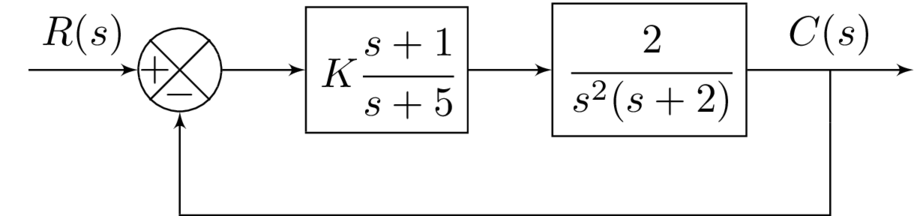
\includegraphics [width=0.7\linewidth]{Q1Diagram67.pdf}
	% \caption{$Q1Diagram67.pdf$}
	\caption{BLock Diagram for B-6-7}
	% Alternative is to typeset the caption myself, which makes more sense to me.
	\label{fig:Q1Diagram67.pdf}
\end{figure}
\begin{align}
& G_{eq}=G_1G_2= K\frac{s+1}{s+5}\frac{2}{s^3+2s^2}
\end{align}

The characteristic equation is $ s^4 + 7 s^3 + 10 s^2 + 2Ks + 2K$, using Routh-Hurwitz Stability Criterion, 
\[\arraycolsep=1.4pt\def\arraystretch{2.2}
\begin{array}{ccc} 1 & 10 & 2\,K\\ 7 & 2\,K & 0\\ 10-\frac{2\,K}{7} & 2\,K & 0\\ \frac{K\,\left(2\,K-21\right)}{K-35} & 0 & 0\\ 2\,K & 0 & 0 \end{array} \]
The value $0 < K < 10.5$, so the critical value of K, $K_{cr} =10.5$. So, locus crosses when K = 0, 10.5. This corresponds to the root locus crossing the imaginary axis when $s=0, \pm 1.73j$. 
\medskip
Furthermore, break away points found by differentiating $dK/ds = 0$ which results in $\displaystyle \frac{(2s(3s^3 + 18s^2 + 31s + 20))}{(s^4 + 7s^3 + 10s^2 + 2s + 2)^2} = 0$
 $6 s^4 + 36 s^3 + 62 s^2 + 40 s=0$. This polynomial has 4 roots at s = $0, -3.7, -1.2 \pm 0.69j$.
 From these 4 roots, there exists 2 real roots at s = 0, -3.7.\hfill \break
 \medskip
 
 The Angles of asymptotes can be computed as $\displaystyle \theta_a=\frac{\pm 180^\circ (2k+1)}{num \ of \ asymptotes} = 0, 60^\circ, 300 ^\circ$. \newline
 \medskip
  The asymptote intersect can be computed as $\displaystyle \sigma_a=\frac{sum \ of \ poles - sum \ of \ zeros}{num \ of \ asymptotes} = ((-7)-(-1))/3 = -6/3 = -2$ \newline
  \medskip
Plotting the root locus in Matlab results in:
\begin{lstlisting}[language = Matlab]
G1 = tf([1,1],[1,5])
G2 = tf([2],[1 2 0 0])
Geq = G1 *G2
rlocus(Geq)
\end{lstlisting}

\begin{figure}
	\centering
	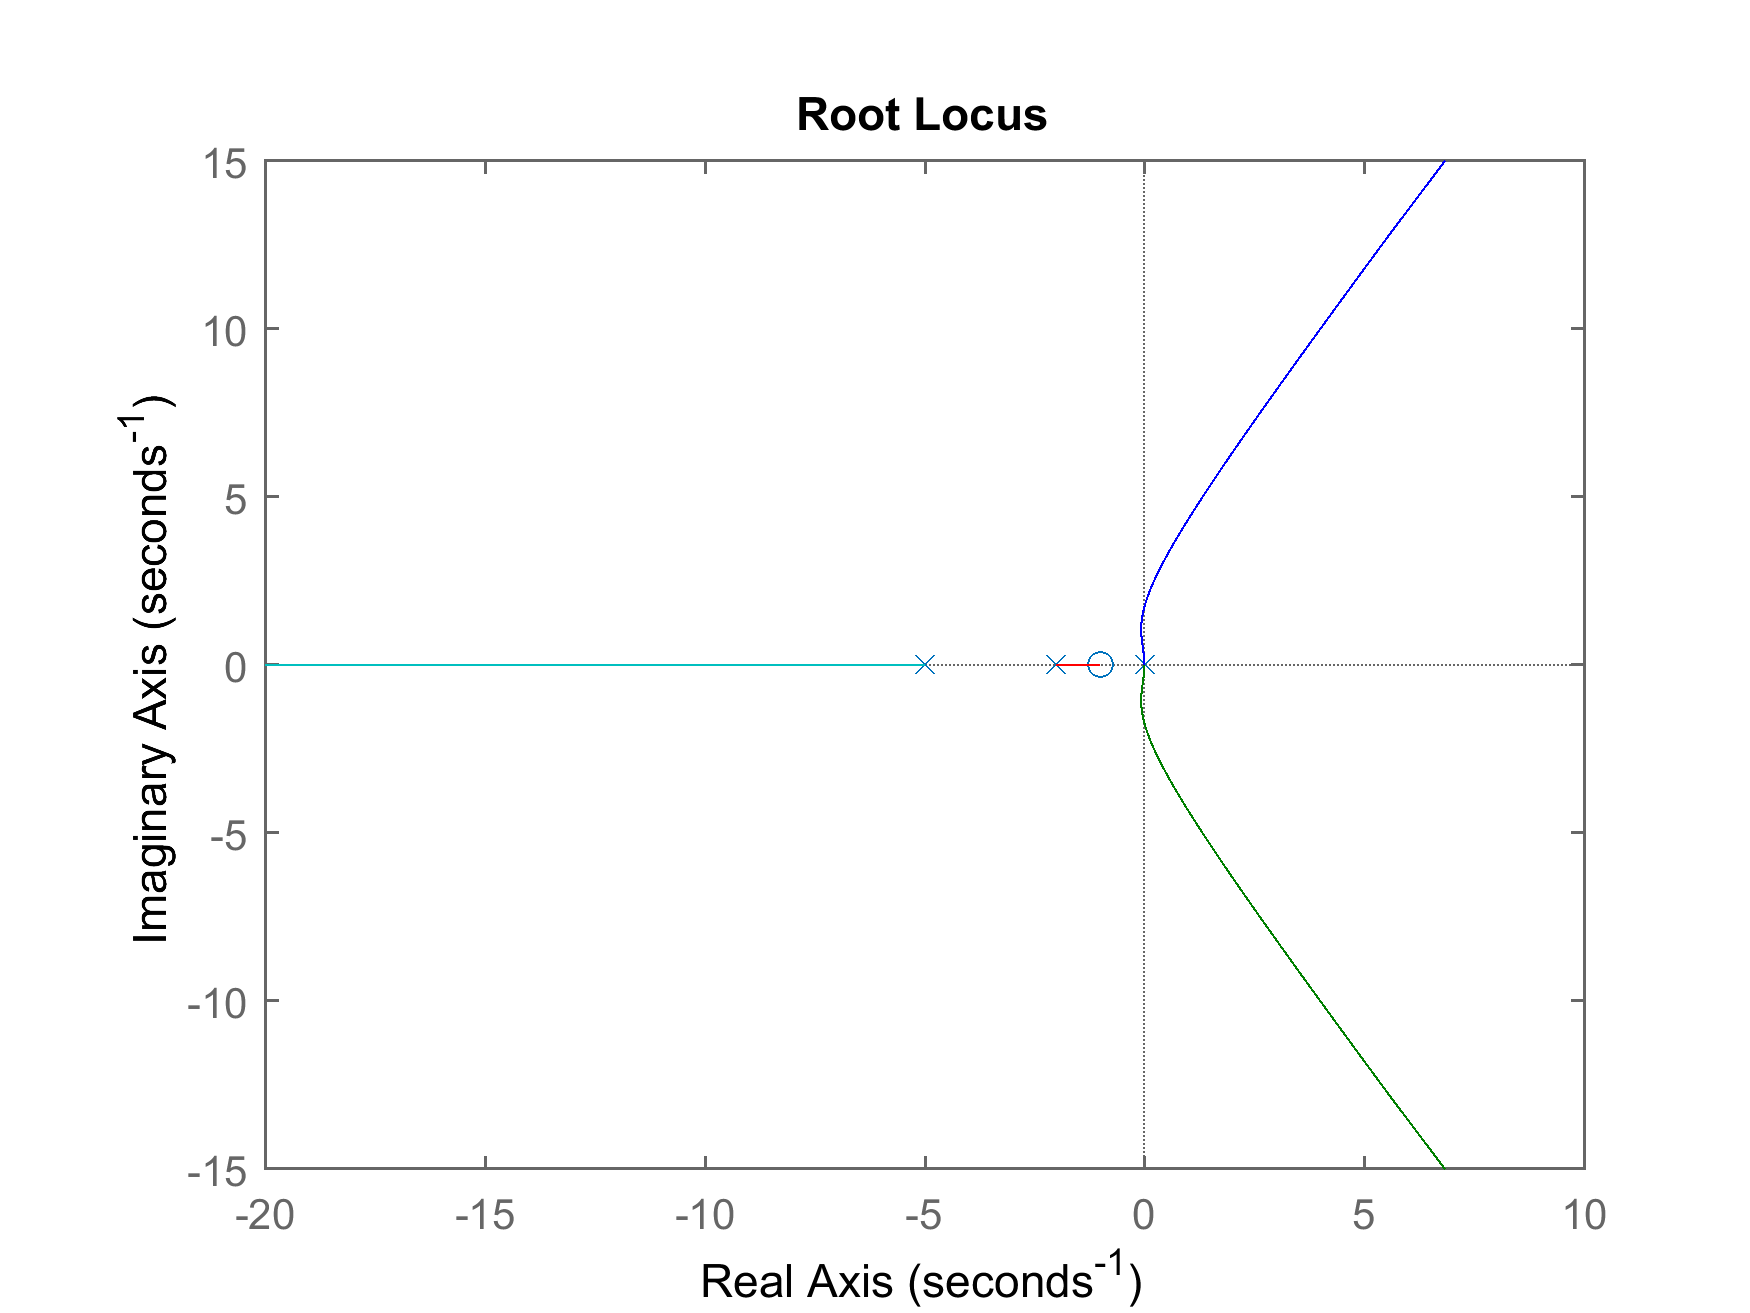
\includegraphics [width=0.7\linewidth]{rlocusQ67NoAnno.png}
	% \caption{$ELEC360A2m_01.pdf$}
	\caption{Root Locus for $G_{eq}=G_1G_2= K\frac{s+1}{s+5}\frac{2}{s^3+2s^2}$}
	% Alternative is to typeset the caption myself, which makes more sense to me.
	\label{fig:ELEC360A2m_01.pdf}
\end{figure}
\begin{figure}
	\centering
	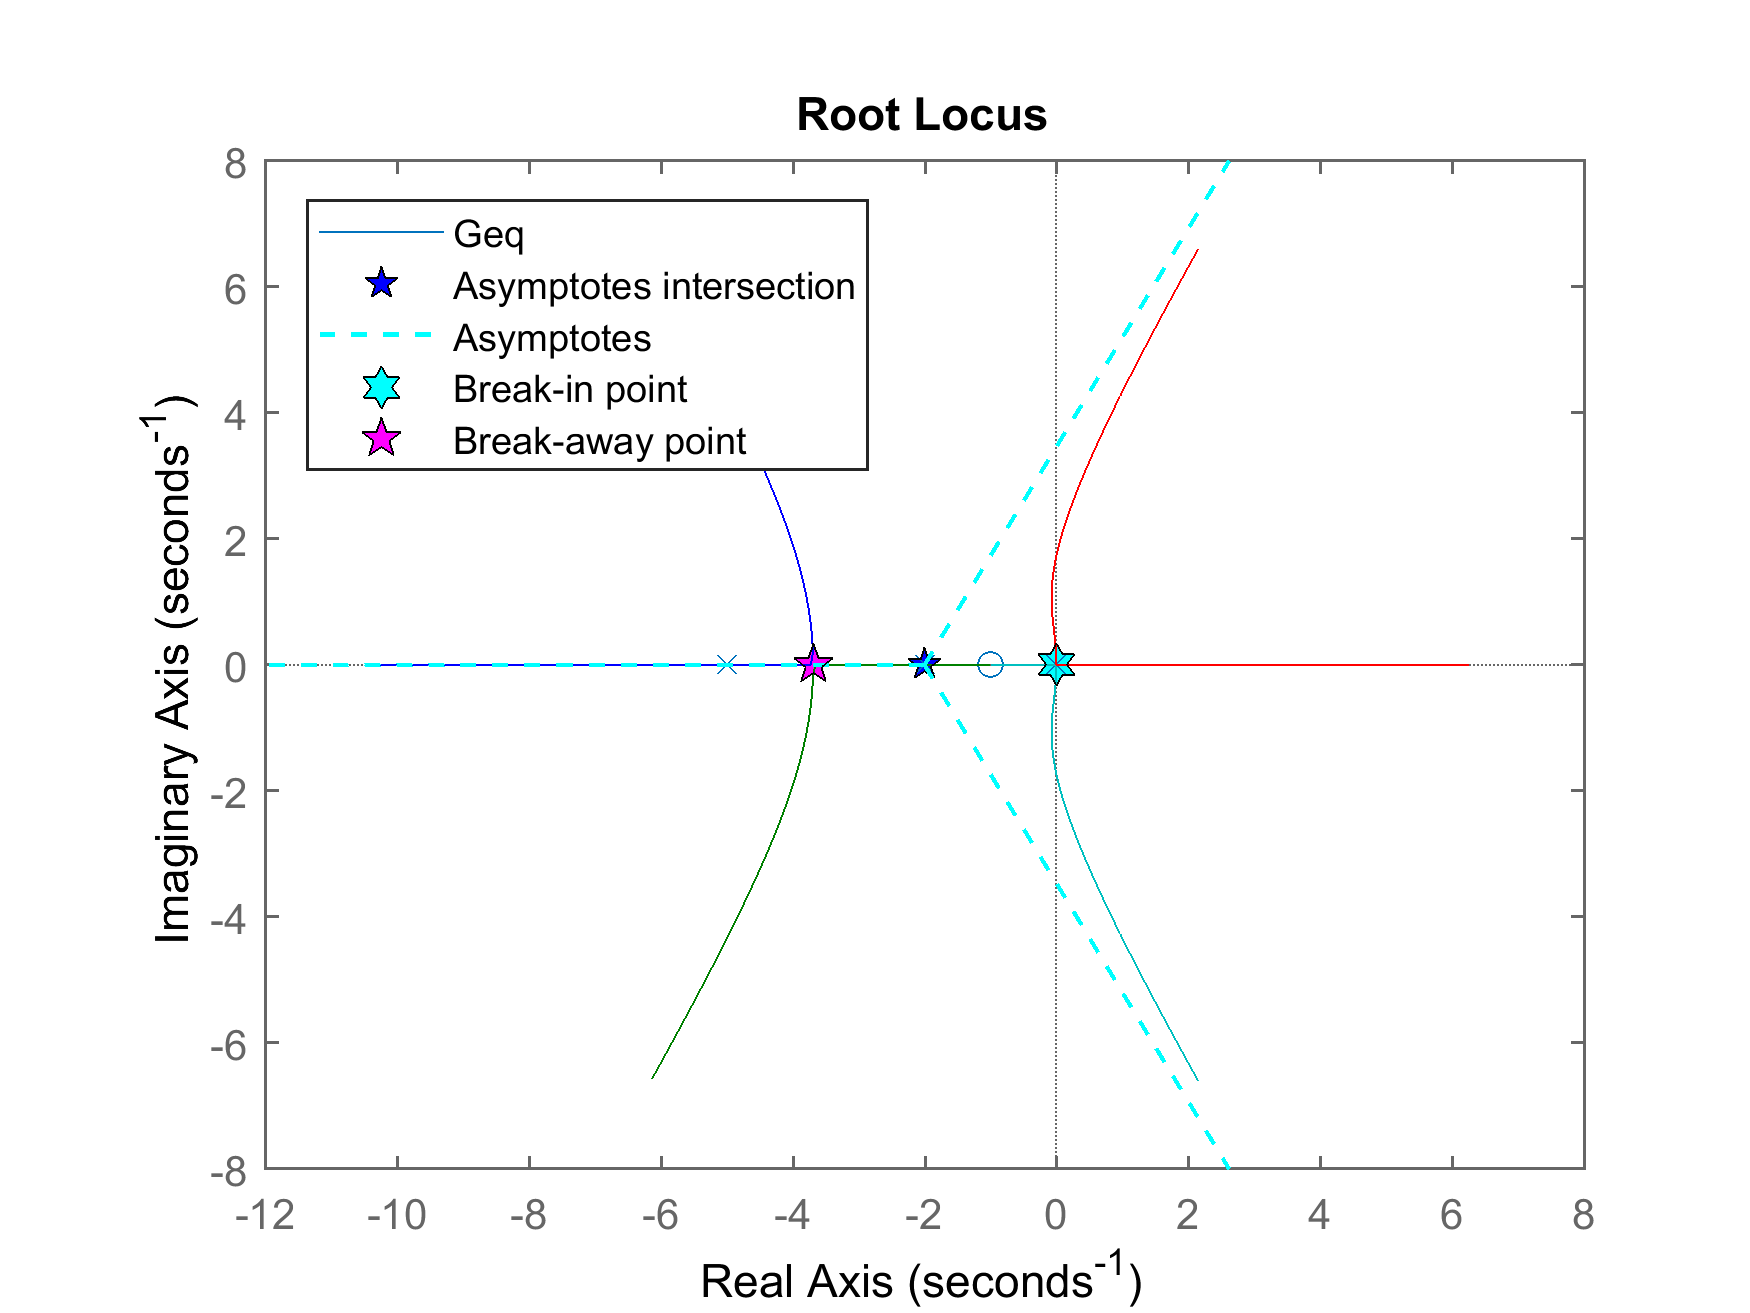
\includegraphics [width=0.85\linewidth]{rlocusQ67Final.png}
	% \caption{$ELEC360A2m_01.pdf$}
	\caption{Root Locus with marked asymptotes and break away points, crossing imaginary axis (K=0, 10.5)}
	% Alternative is to typeset the caption myself, which makes more sense to me.
	\label{fig:ELEC360A2m_Edge.pdf}
\end{figure}
\newpage

\subsection*{Question 2: B-6-14}

\begin{par}
	Since $\xi = 0.5$, $\theta=\cos^{-1}(\xi)=60^o$, then since $\sin(\theta)= \sqrt(3/2)$ and $\cos(\theta)= 1/2$. $s= -\sigma/2 + j \omega_d$, normalizing gives $s = -x + j\sqrt(3)x$
\end{par} \vspace{1em}
\begin{figure}[h]
	\centering
	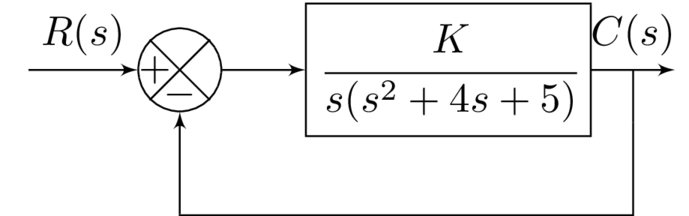
\includegraphics [width=0.5\linewidth]{Q2Diagram614.pdf}
	% \caption{$Q2Diagram614.pdf$}
	\caption{Block Diagram for 6-14}
	% Alternative is to typeset the caption myself, which makes more sense to me.
	\label{fig:Q2Diagram614.pdf}
\end{figure}


% See %\href{https://www.wolframalpha.com/input/?i=(-x+%2B+i%5Csqrt(3)x)%5E3%2B4(-x+%2B+i%5Csqrt(3)x)%5E2%2B5(-x+%2B+i%5Csqrt(3)x)%2BK%3D0}{https://www.wolframalpha.com/input/?i=(-x+%2B+i%5Csqrt(3)x)%5E3%2B4(-x+%2B+i%5Csqrt(3)x)%5E2%2B5(-x+%2B+i%5Csqrt(3)x)%2BK%3D0}

\begin{par}
\begin{align*} & 1 + \frac{K}{s^3+4s^2+5s} = s^3+4s^2+5s+K =0 \\ & = (-x + j\sqrt(3)x)^3+4(-x + j\sqrt(3)x)^2+5(-x + j\sqrt(3)x) + K = 0 \\ & = K +8x^3+(-8-8j\sqrt(3))x^2+j5\sqrt(3)x-5x=0 \\ \end{align*}
\end{par} \vspace{1em}
\begin{par}
Equating real and imaginary parts
\end{par} \vspace{1em}
\begin{par}
\begin{align} & 8x^3-8x^2-5x+ K = 0 \\ & -j8\sqrt(3)x^2+j5\sqrt(3)x=0 \end{align}
\end{par} \vspace{1em}
\begin{par}
Solving for x, gives $x=5/8$
\end{par} \vspace{1em}
\begin{par}
$ 8(5/8)^3-8(5/8)^2-5(5/8)+ K=0$
\end{par} \vspace{1em}
\begin{par}
leads to $K=\frac{275}{64}=4.296875$
\end{par} \vspace{1em}
\begin{par}
Plot root locus
\end{par} \vspace{1em}
\begin{lstlisting}[language = Matlab]
G = tf([1],[1 4 5 0])
rlocus(G)
sgrid
\end{lstlisting}
\color{black}    
\begin{figure}[h]
	\centering
	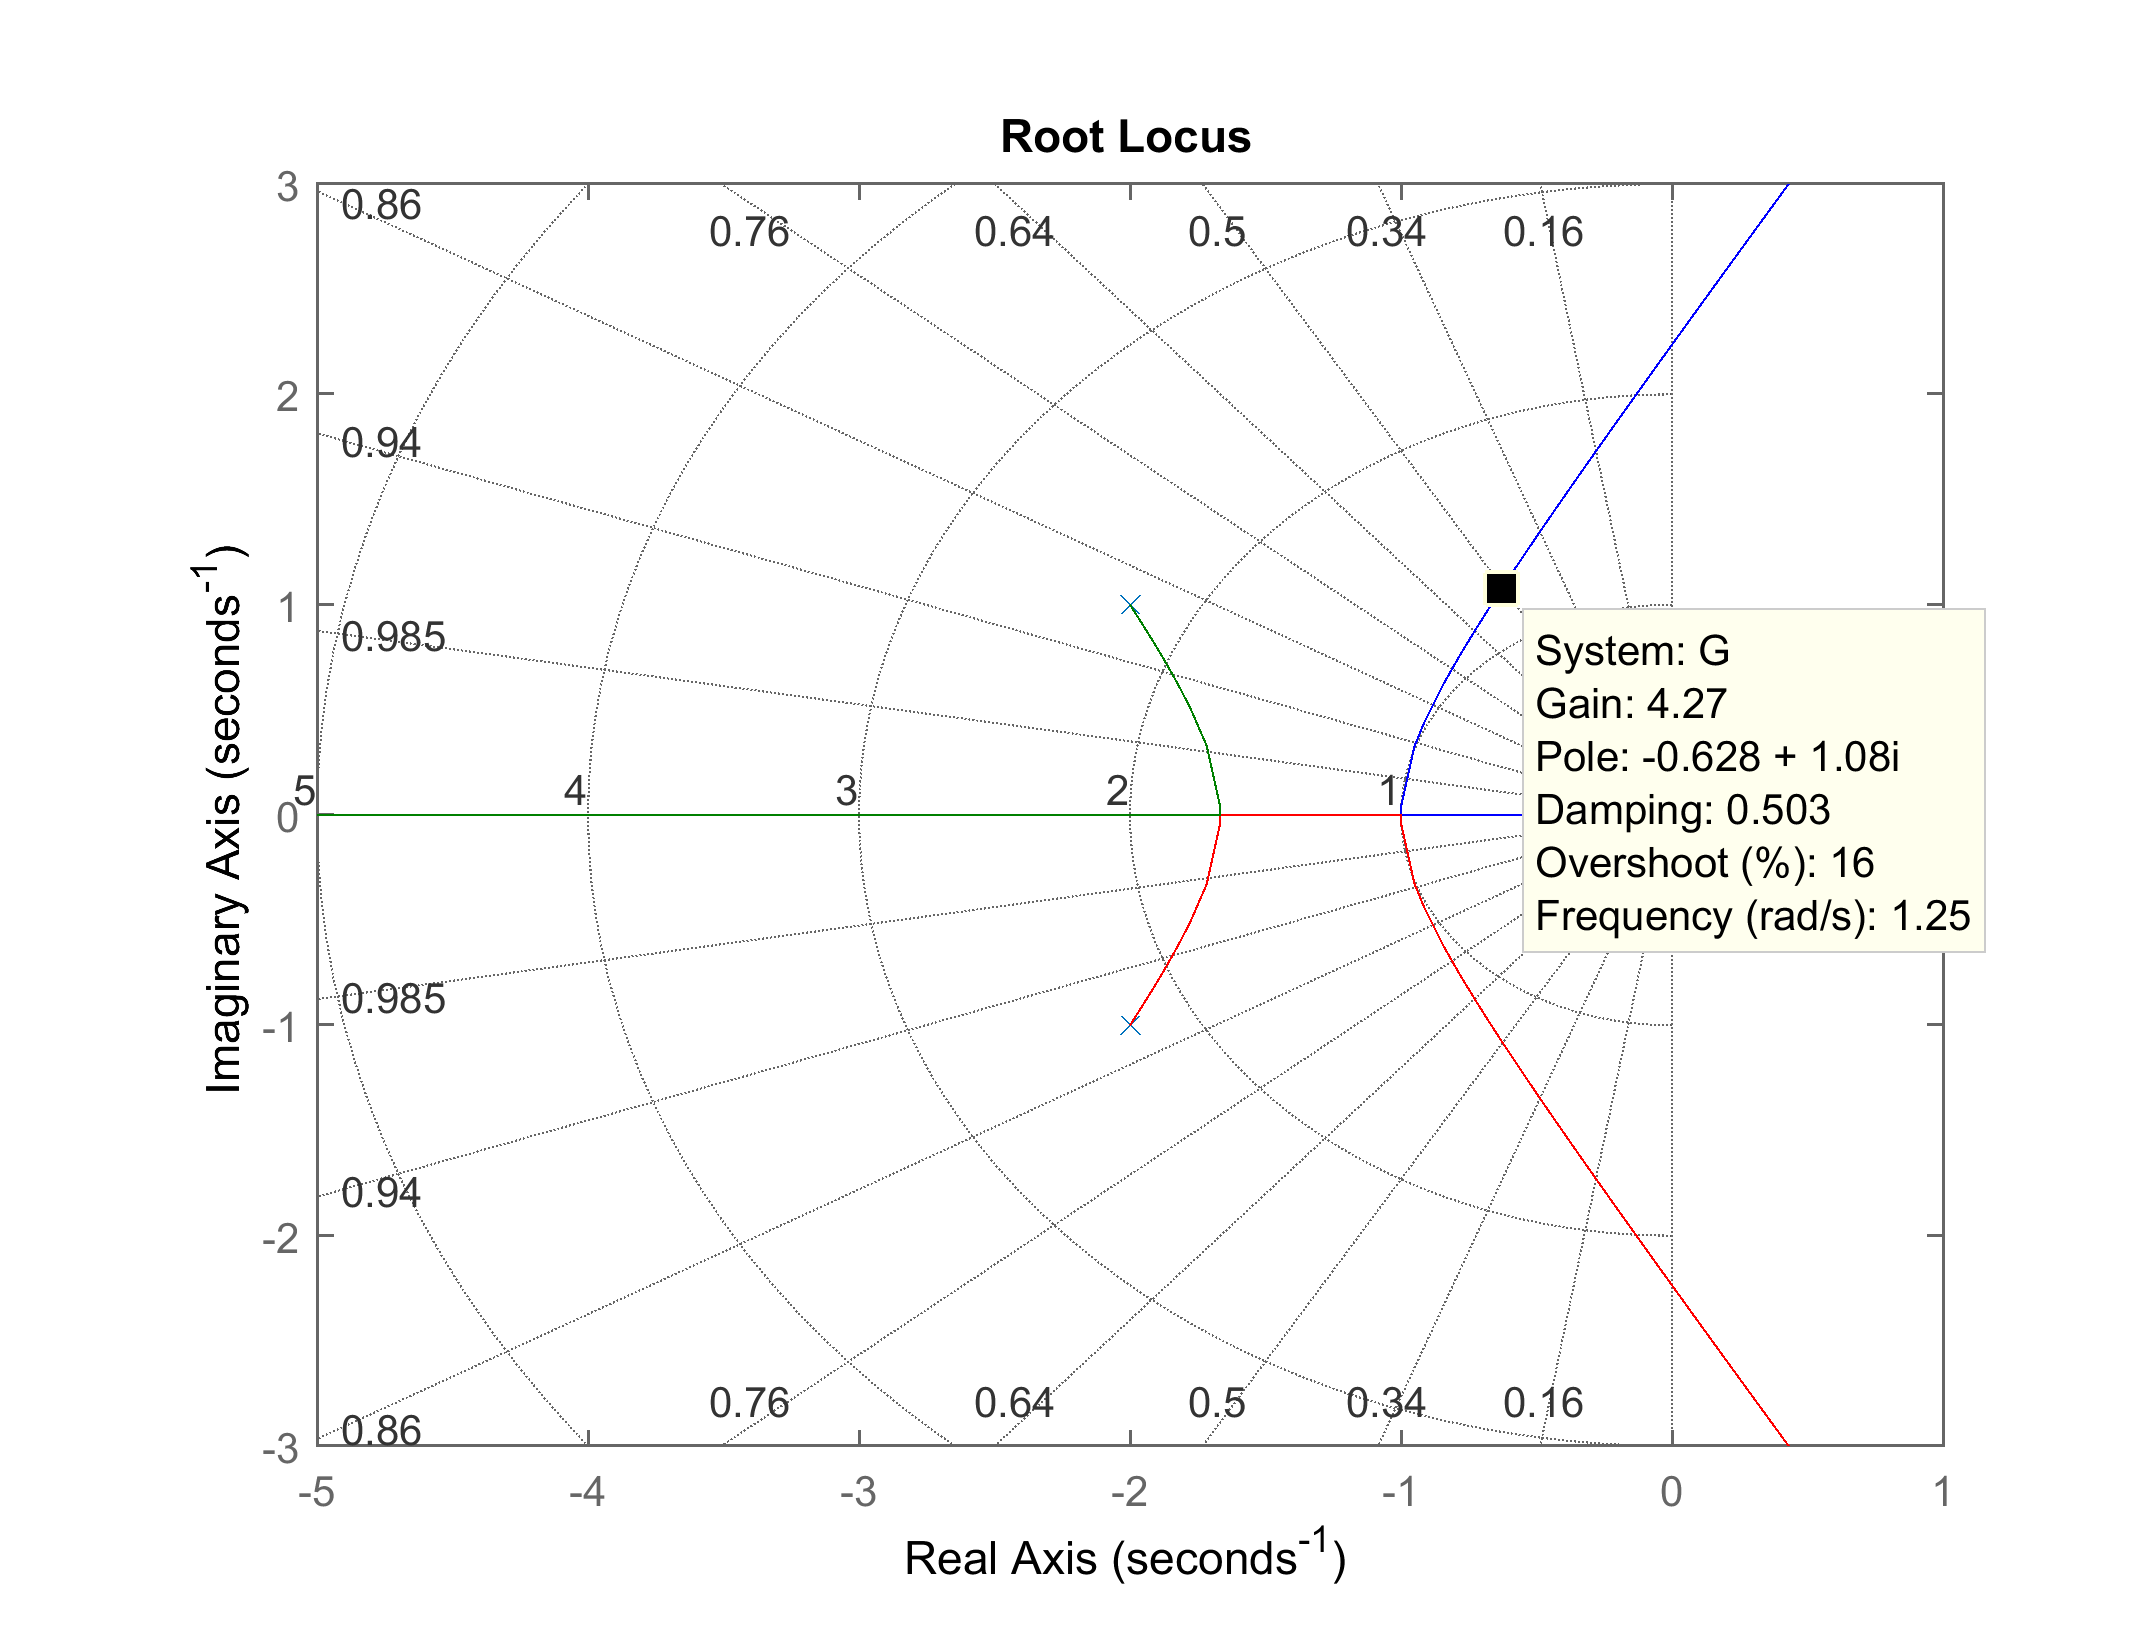
\includegraphics [width=0.75\linewidth]{rlocusQ614Anno.png}
	% \caption{$ELEC360A2m_02.pdf$}
	\caption{Root Locus for B-6-14}
	% Alternative is to typeset the caption myself, which makes more sense to me.
	\label{fig:ELEC360A2m_02.pdf}
\end{figure}
\begin{par}
from the root locus, the gain is about K = 4.27
\end{par} \vspace{1em}
\begin{par}
Plot step response, take C(s) / R(s)
\end{par} \vspace{1em}
\begin{lstlisting}[language = Matlab]
Geq = feedback(G,1)
GeqS = Geq*4.2969
% take coefficients from feedback function
num = [0 0 0 4.2969]
den = [1 4 5 4.2969]
step(num,den)
\end{lstlisting}
    
\begin{figure}[H]
	\centering
	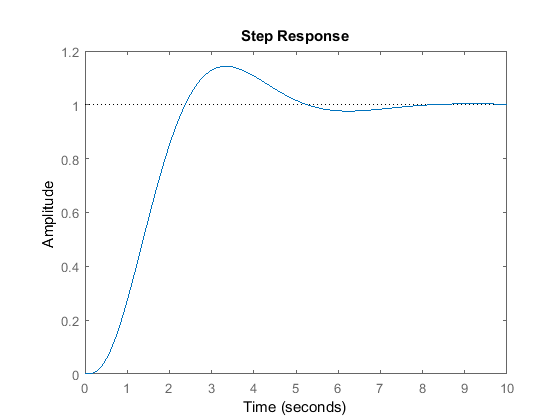
\includegraphics [width=0.75\linewidth]{ELEC360A2m_03.png}
	% \caption{$ELEC360A2m_03.pdf$}
	\caption{Unit Response for B-6-14}
	% Alternative is to typeset the caption myself, which makes more sense to me.
	\label{fig:ELEC360A2m_03.pdf}
\end{figure}


\subsection*{Question 3 B-6-16}

\begin{figure}[H]
	\centering
	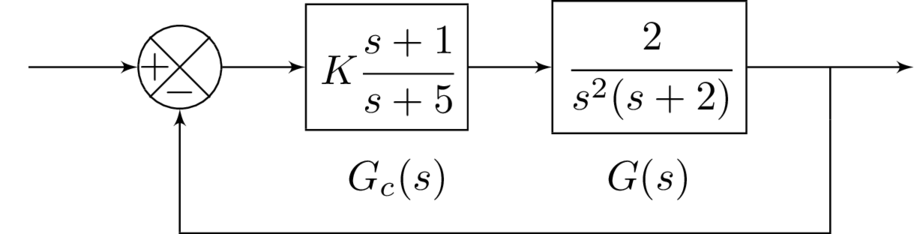
\includegraphics [width=0.7\linewidth]{Q3Diagram616.pdf}
	% \caption{$Q3Diagram616.pdf$}
	\caption{Block Diagram for B-6-16}
	% Alternative is to typeset the caption myself, which makes more sense to me.
	\label{fig:Q3Diagram616.pdf}
\end{figure}

%\begin{lstlisting}[language = Matlab]
%G1 = tf([1],[1 2 0])
%\end{lstlisting}
The poles must be at the closed-loop poles are located at
$s = -2 \pm j2$, the transfer function in terms of K, and T.
\begin{align*}
& \frac{C(s)}{R(s)}=\frac{K(Ts+1)}{s(s+2)+K(Ts+1)} \\
& s(s+2)+KT(s+1)=(s+2+j2)(s+2-j2) \\
& s^2+(2+KT)s+KT=s^2+4s+4 \\
& (2+KT)s = 4s, \quad KT = 4
\end{align*}
$K=8$ and $2+KT=4$, so $T=0.25$

\subsection*{Question 4, B-6-17}

The compensator must have a pole at -4, since $\sin^{-1}(2/4)=30^o$. 
\begin{align*}
& G_c(s) = K\frac{s+2}{s+4} \\
& \text{The angle deficiency is } 180^o-120^o-90^o=-30^o
\end{align*}
\begin{figure}[H]
	\centering
	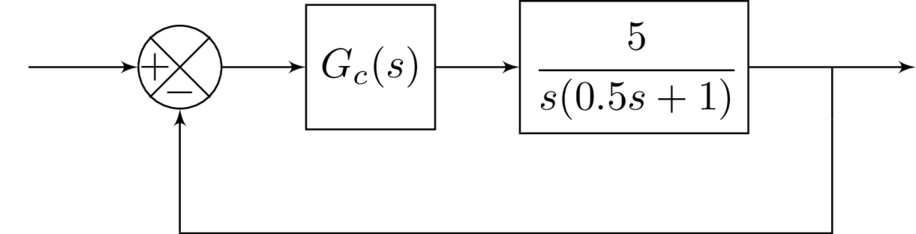
\includegraphics [width=0.7\linewidth]{Q4Diagram617.pdf}
	% \caption{$Q4Diagram617.pdf$}
	\caption{Block Diagram 6-17}
	% Alternative is to typeset the caption myself, which makes more sense to me.
	\label{fig:Q4Diagram617.pdf}
\end{figure}
The gain of the compensator can be found using: Figure \ref*{fig:polesZeroes.pdf}
\begin{align*}
& \left| K \frac{s+2}{s+4} \times \frac{5}{0.5s(s+2)} \right|_{s=-2+j2\sqrt(3)}=1 \\
& K = 8/5 = 1.6 
\end{align*}
%plotting uncompensated step function
\begin{lstlisting}[language = Matlab]
numC = [5]
denC = [0.5 1 5]
step(numC,denC)
hold on
num = [8 16]
den = [0.5 3 12 16]
step(num,den)
legend('Original Step Response', 'Compensated Step Response')
\end{lstlisting}
\begin{figure}[H]
	\centering
	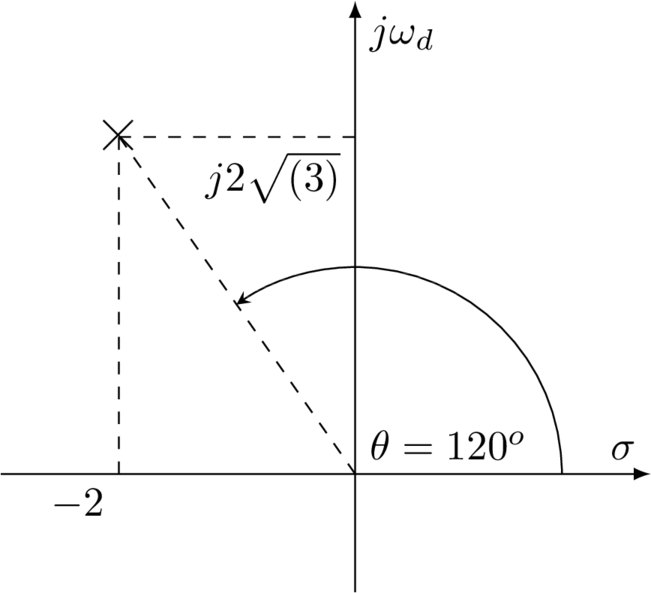
\includegraphics [width=0.75\linewidth]{polesZeroes.pdf}
	% \caption{$polesZeroes.pdf$}
	\caption{Finding the location of the pole}
	% Alternative is to typeset the caption myself, which makes more sense to me.
	\label{fig:polesZeroes.pdf}
\end{figure}


\begin{figure}[H]
	\centering
	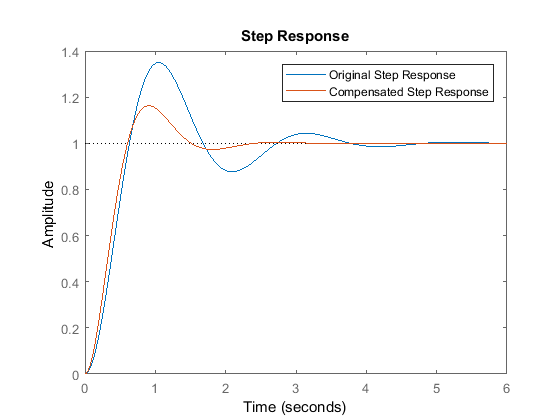
\includegraphics [width=0.75\linewidth]{ELEC360A2m_04.png}
	% \caption{$ELEC360A2m_04.pdf$}
	\caption{Compensated Step Response vs Original Step Response}
	% Alternative is to typeset the caption myself, which makes more sense to me.
	\label{fig:ELEC360A2m_04.pdf}
\end{figure}

\newpage
\subsection*{Question 5, B-6-20}

\begin{align} & \text{Ch. Eqn Original} = s(s+10)(s+20)+820 = s^3 + 30s^2+200s+820 \\ & s=-3.6 \pm j4.8, s=-22.8 \\ & G\_c(s) = \hat{K}\_c\beta\frac{Ts + 1}{\beta Ts+1} \end{align}

\begin{figure}[h]
	\centering
	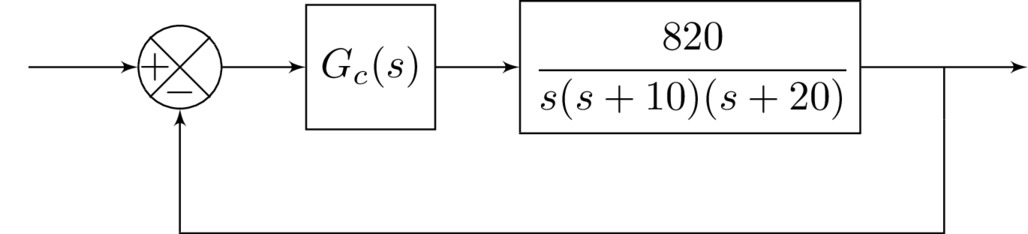
\includegraphics [width=0.7\linewidth]{Q5Diagram620.pdf}
	% \caption{$Q5Diagram620.pdf$}
	\caption{}
	% Alternative is to typeset the caption myself, which makes more sense to me.
	\label{fig:Q5Diagram620.pdf}
\end{figure}

If the poles of the compensator function as placed near the origin, the angle contribution will be very small and impact the system response will be small.
\begin{align} 
& -5^o < \angle\left( \frac{s+ 1 / T}{s+ 1 /(\beta T)} \right) < 0^o \\
& K \approx 1, \beta = 10, T = 8 \\ & G\_c(s) = 10\frac{8s+1}{80s+1}= \frac{s+0.125}{s+0.0125} \end{align}

Since the angle contribution is about $-0.8713^o$, which is acceptable given the design specifications.
Computing velocity error $K_v =\lim\limits_{s \rightarrow 0}sG(s)=41$ \hfill \break


The characteristic equation for the new system is: $s^4 + (2401*s^3)/80 + (1603*s^2)/8 + (1645*s)/2 + 205/2$

The roots of the polynomial are: $s= -22.797, -3.5435 + 4.7344j,-3.5435-j4.7344, -0.12857$ \hfill \break $\omega_n=|-3.5435 + j4.7344|=5.913622$. \hfill \break

Since $\omega_n=5.913622884$, the compensator system has an adjustment of about 1.44 \%

\subsection*{Question 6, B-7-4}
\begin{align} 
& G(s) =\frac{10(s^2+0.4s+1)}{(s(s^2+0.8s+9))} \\
& G(s) =10\frac{s+(0.2+j2\sqrt{6})s+(0.2-j2\sqrt{6}}{s(s+(0.4+j2.97321))(s+(0.4-j2.97321))} \\
& G(s) = 10 \frac{1}{9}\cfrac{s^2+0.4s+1}{s(\frac{s^2}{9}+\frac{0.8s}{9}+1)} = G(j\omega) = \frac{10}{9}\cfrac{(j\omega)^2+0.4(j\omega)+1}{j\omega(\frac{(j\omega)^2}{9}+\frac{0.8(j\omega)}{9}+1)}
\end{align}
constant of $10/9$, zeroes at = $-0.2-j2\sqrt{6},-0.2+j2\sqrt{6}$, poles at = $-(0.4-j2.97321), -(0.4+j2.97321)$
% figure out how to manually plot this graph later
\begin{lstlisting}[language = Matlab]
num = [10 4 10]
den =[1 0.8 9 0]
Gc = tf(num,den)
bode(Gc)
\end{lstlisting}
    
\begin{figure}[h]
	\centering
	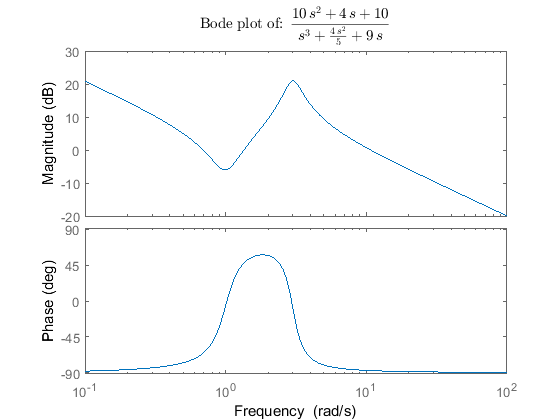
\includegraphics [width=0.7\linewidth]{ELEC360A2m_05.png}
	% \caption{$ELEC360A2m_05.pdf$}
	\caption{Bode Plot for 7-4}
	% Alternative is to typeset the caption myself, which makes more sense to me.
	\label{fig:ELEC360A2m_05.pdf}
\end{figure}


\end{document}
    
